\documentclass[twoside,letterpaper,twocolumn]{article}

%%%%%%%%%%%%%%%%%%%%%%%%%%%%%%%%%%%%%%%%%%%%%%%%%%%%%%%%%%%%%%%%%%%%%%
% Package with format specifications for the 9th CISBGf
\usepackage{cisbgf}

%%%%%%%%%%%%%%%%%%%%%%%%%%%%%%%%%%%%%%%%%%%%%%%%%%%%%%%%%%%%%%%%%%%%%%
% MANDATORY PARAMETERS

% Setting the title
\title{Seismological Data Management of BRASIS - BRAzilian Integrated
Seismological Network}

% Setting the authors
\author{Bruno Colla\c{c}o, Jackson Calhau, Marlon Pirchiner, Marcelo
Assump\c{c}\~{a}o, Centro de Sismologia - IAG/IEE - USP, Brazil }

% Setting the headings
\headauthor{Pirchiner, Colla�o, Calhau et al.}
\headtitle{Seismological Data Management}

%%%%%%%%%%%%%%%%%%%%%%%%%%%%%%%%%%%%%%%%%%%%%%%%%%%%%%%%%%%%%%%%%%%%%%
%%%%%%%%%%%%%%%%%%%%%%%%%%%%%%%%%%%%%%%%%%%%%%%%%%%%%%%%%%%%%%%%%%%%%%
\begin{document}

\maketitle

\begin{abstract}

This paper discusses the benefits of jointly inverting for inelastic absorption and convolution
in daily processing flows. Efficiency and stability are shown to be mainly a consequence of a 
proper treatment of the (quasi) null space associated with the combination of these two processes rather
than to the original signal to noise ratio available.
For the sake of clarity, singular value decomposition is used for discussing and 
constructing the pseudo-inverse for the combined process. A simplified assumption of a time-dependent
absorption model is used. 

\end{abstract}

\section{Introduction}

Seismic processing is divided into many independent steps. Each one of these steps deals 
with different processes seismic waves undergo before being recorded.
The reason for treating a particular process independently may be related to the need for 
focusing and optimizing the results with a proper choice of 
parameters, resources, etc. However, some of these steps involve the inversion of an operator in an ill 
posed/conditioned problem and this may require a laborious handling of 
the stability which can be achieved via the knowledge of the spectrum of the 
associated operator. Usually this is a trial and error method performed 
until an acceptable signal to noise ratio is achieved. 

Deconvolution and absorption compensation are examples of this class of processes. The proper choice of
a white noise level may be essential for the stability in the deconvolution and
the level of amplification in high frequencies is critical for absorption compensation.
Unfortunately, these two processes cannot be optimally treated in a step by 
step way. Since the null space of the combined process is generally not simply related
to the null space of the individual processes it may be worth to adopt a unified
approach. This is specially critical when signal to noise ratio is low.

Usually, absorption is treated after deconvolution when the signal to noise ratio has already
been degraded in the high frequency range due to an apparently optimal choice of white noise. That the level
of white noise is not optimal is not easily seen until one effectively tries to recover the high 
frequency portion of the spectrum as in the absorption compensation.

A very common practice is to break absorption into attenuation and phase leaving the attenuation compensation
for a post-stack step where it is supposed that the signal to noise ratio has been enhanced. This approach is 
artificial and do not help seismic processing pre-stack steps like velocity analysis to reach a higher
level of resolution. It is shown here that pre-stack compensation of absorption may be done with an easy control
of stability in conjunction with deconvolution providing a better suited data. 


\section{A joint operator for deconvolution and absorption}

A seismic trace $s(t)$ can be described as the convolution of a pulse $p(t)$ with an earth
impulsive response $e(t)$ that may be decomposed into a local reflectivity $r(t)$ and 
a causal absorption filter $A(t,\tau)$ in the following way, 
\begin{equation}
 s(t)\,=\,p(t)\ast \int_0^{\infty}A(t,\tau)r(\tau)d\tau
\end{equation}
with $t$ and $\tau$ standing for current and travel times and
$\ast$ is convolution. This expression may be rewritten as,
\begin{equation}
 s(t)\,=\int_0^{\infty}\left[ \int_0^{\infty}p(t-t')A(t',\tau)dt'\right] r(\tau)d\tau
\end{equation}
where the joint operator of convolution and absorption is inside brackets.

A discrete version of the equation above can be written as follows,
\begin{equation}
 \vec s = \mathbf{P}\mathbf{A}\, \vec r
\end{equation}
where $\vec s$ has the samples of the recorded trace, $\mathbf{P}$ is a low diagonal matrix with the
samples of the causal pulse $p_i$ displayed in the columns as,
\begin{equation}
 P_{nm}\,=\,p_{n-m}\,\, ,
\end{equation}
and $\mathbf{A}$ is also a low diagonal matrix representing the causal effect 
of absorption for a given travel time $\tau_m$ as,
\begin{equation}
 A_{nm}\,=\,\mathcal{A}_{n,\tau_m},
\end{equation}
with $\mathcal{A}$ based in a phenomenological model for absorption here taken 
from Futtermann's absorption model (1962) expressed as,
\begin{equation}
 \mathcal{A}(t,\tau)\,=\,\int_{-\infty}^{\infty}e^{2\pi i ft}e^{-\frac{\pi f\tau}{Q}\left(1 + \frac{2i}{\pi}
\log{f/f_0}\right)}df \,\,\, ,
\end{equation}
parametrized by the quality factor $Q$ and a reference frequency $f_0$.

The joint operator for convolution and absorption is also causal, with a discrete representation 
as a low diagonal matrix exhibiting filtered versions of the pulse in columns, each column associated 
to a different travel time.



\section{A pseudo-inverse for the processes}

Deconvolution and absorption compensation are often characterized by an ill posed and/or an ill
conditioned inversion problem. They demand some kind of regularization which can be easily made via
singular value decomposition (SVD) (1965) of the associated matrix. A common approach 
consists of grouping singular values according to their magnitude so as to apply a particular treatment 
to each one. For example, there could be a subset of numerically stable (larger) singular values, a 
subset of numerically unstable singular values (quasi null), and a null space. A pseudo-inverse is commonly
build with the inversion of the former, a dumped or controlled inversion of the second group, and the 
same null space. 

Deconvolution and absorption compensation usually do not share the same set of singular vectors in which case
an optimal pseudo-inverse for the combined process would be easily constructed after treating each process
separately. More precisely, given the SVD of the convolution operator $\mathbf{P}\,=\,\mathbf{U}_P\,\Lambda_P\,\mathbf{V}^H_P$ and
the absorption operator $\mathbf{A}\,=\,\mathbf{U}_A\,\Lambda_A\,\mathbf{V}^H_A$, the requirement for successfully 
treating the operator $\mathbf{PA}$ via the analysis of $\mathbf{P}$ and $\mathbf{A}$ separatelly would be that 
$\mathbf{V}^H_P\,\mathbf{U}_A\,=\,\mathbf{I}$ where $\mathbf{I}$ is the identity. In this case 
$\mathbf{PA}\,=\,\mathbf{U}_P\,\Lambda_P\,\Lambda_A\,\mathbf{V}^H_A$ and an optimal subdivision of subspaces holds
for both operators since $ \Lambda_{PA}\,=\,\Lambda_P\,\Lambda_A$.

An analysis of current seismic processing practice based on what was said above would conclude that any attempt to
regularize one of the processes independently will likely be amplifying the instability of the other. In other words,
most of the hard work required for defining an acceptable absorption compensation could be avoided if deconvolution 
had not been applied before. Building a pseudo-inverse for the joint operator for convolution and absorption brings 
the advantage of optimally controlling the sensitive subspaces and reducing cycle time.

\section{A real data example}

For the sake of comparison, figure 1 shows a small window of a stacked section where \textit{a}) absorption
compensation was applied after stacking, \textit{b}) a 1-40 Hz bandpass filter was applied on the section 
shown on \textit{a}), and \textit{c}) deconvolution and absorption compensation were applied as a single 
pre-stack process. 

Figure 1\textit{a} shows the usual signal to noise ratio one obtains
without a strict control of amplification of the higher frequency range of the spectrum. In this case, 
signal has its bandwidth mostly restricted to the low end of the spectrum and noise (multiples) spectrum
is broader. 

In the step by step processing, absorption compensation is often followed by bandpass filters in an 
attempt to attenuate the high frequency components of the noise as shown in Figure 1\textit{b}. 
This procedure does not alter the signal to noise ratio on the bandwidth of the signal. Absorption 
is not characterized by a convolutive operator. Thus, its effect on the frequency content of the data is not 
straightforwardly understood.

\begin{figure}[h!]
  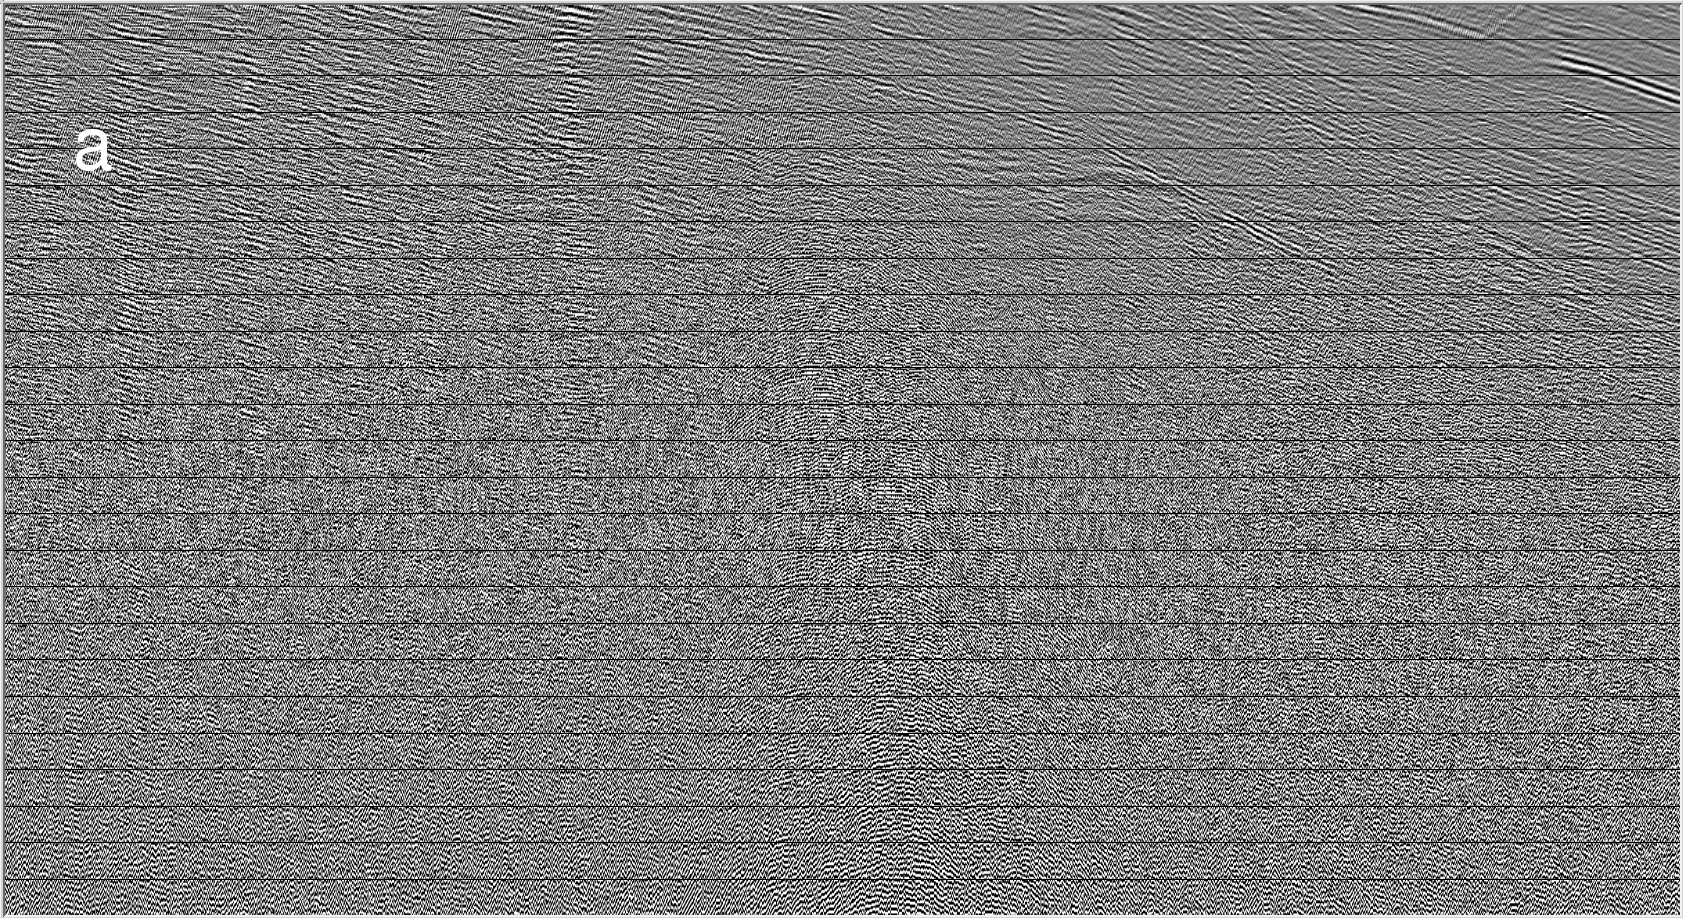
\includegraphics[width=8cm]{images/Filtro_pos_empilhamento.jpg}
  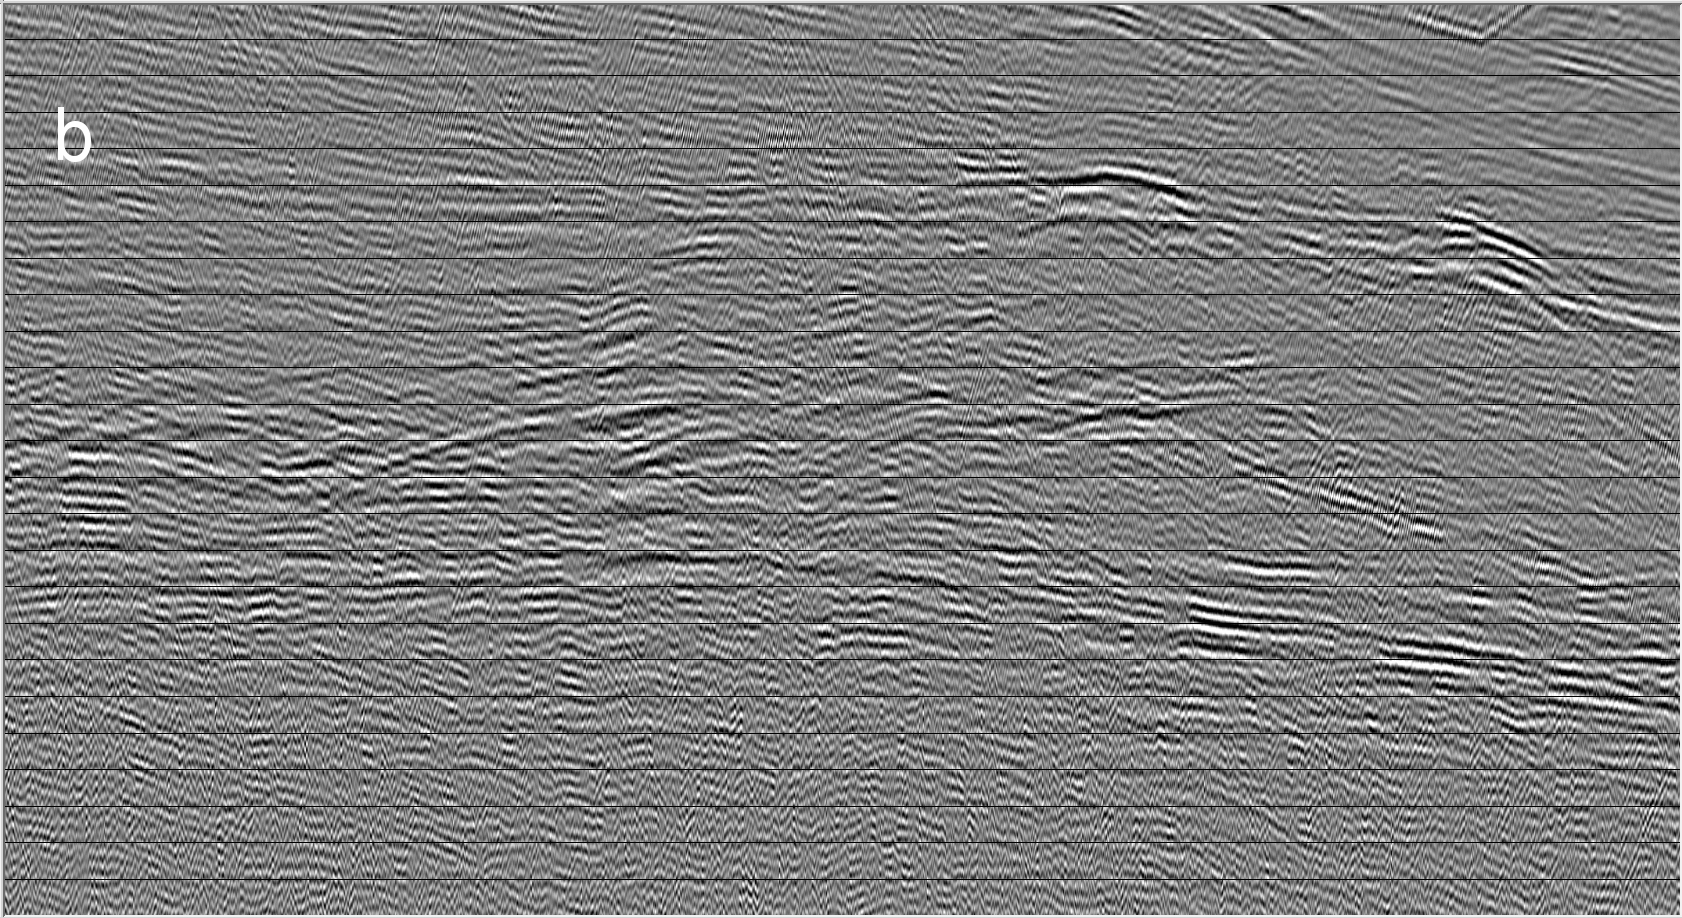
\includegraphics[width=8cm]{images/Filtro1-2-25-40.jpg}
  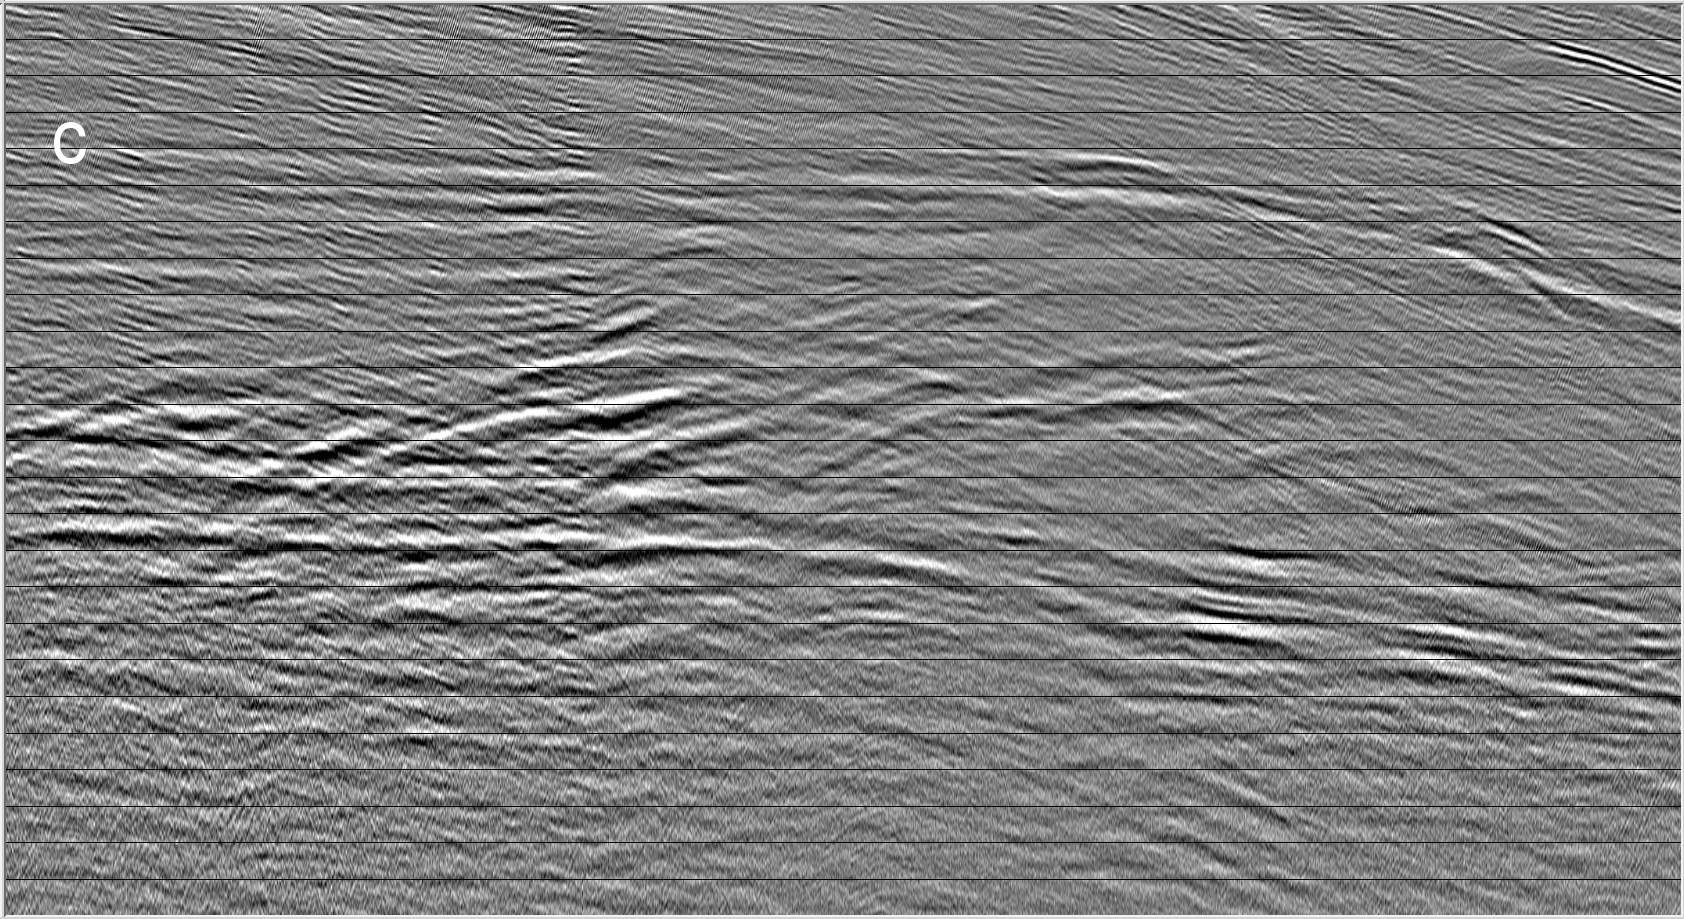
\includegraphics[width=8cm]{images/Filtro_PA.jpg}
 \caption[Figure 1]{\textit{a}) On top, for comparison, the resulting section after the
step by step deconvolution and (pos-stack) absorption compensation; \textit{b}) in the middle, 
the section shown on top after a 1-2-25-40 Hz trapezoidal bandpass filter;  \textit{c}) Below, the
same window of the stacked section after (pre-stack) jointly compensating for absorption and 
deconvolution. Gain was applied to allow for comparison of signal to noise ratio.}
\end{figure}

Figure 1\textit{c}) has a much more clear definition of the geological structures, without 
the undesired change in the high to low frequency content ratio. The inversion of the combined operator
has done a more adequate treatment of the unstable side of the combined operator, resulting in a more balanced
signal to noise ratio in different frequency ranges. 

The SVD parametrization was the same in all figures. Since absorption compensation alter the 
level of amplitudes, gain was applied for better visualization of the signal to noise ratio.

To have an idea of the stability of the joint compensation for absorption and deconvolution
in pre-stack data, figure 2 shows a shot \textit{a}) before and \textit{b}) after 
compensation. It is clear that the usual amplification of high frequency noise is not 
present. In fact, the frequency content of compensated data is only slightly shifted as 
compared to the original shot. Although limitations on the spectrum was not desired, this 
result is a consequence of frequency content limitations on the pulse used for the combined 
inversion. On one hand, the proposed technique did not improved our estimate of the higher frequency 
content of reflectivity remarkably. However, on the other hand, we have achieved the 
best possible equalization of the spectrum without the inconvenient trial and error 
time consuming process of handling the noise amplifyied through absorption compensation.

\begin{figure}[h!]
  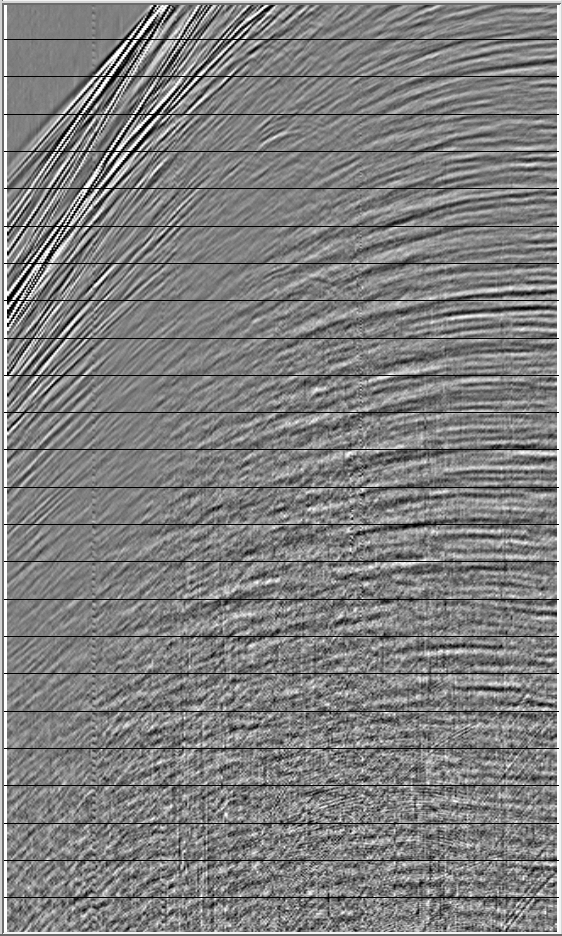
\includegraphics[width=4cm]{images/tiro_original.png}
 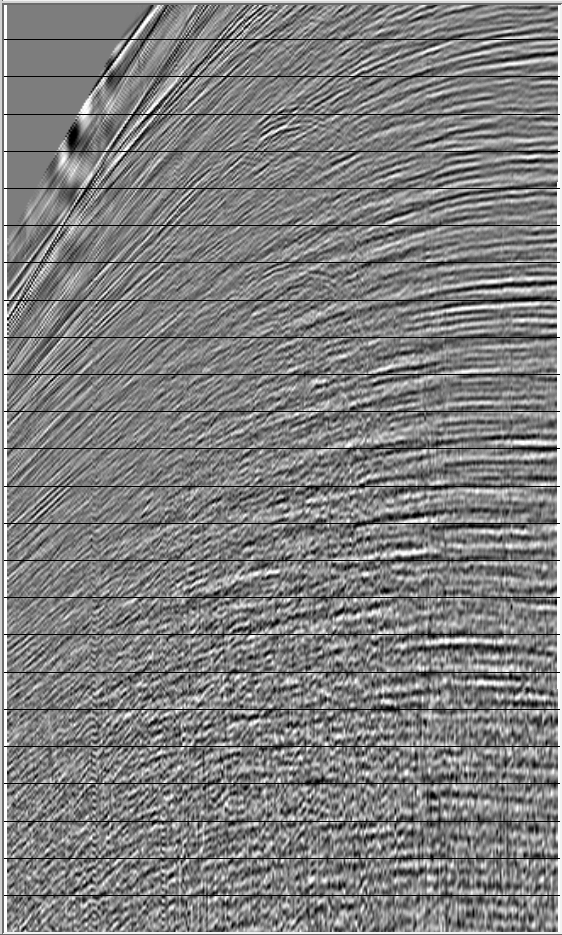
\includegraphics[width=4cm]{images/Filtro_tiro.png}
 \caption[Figure 2]{\textit{a}) Left, a shot record before deconvolution and right, 
  \textit{b}) the same shot after jointly compensating for absorption and deconvolution. Gain was 
  applied to allow for appraisal of the signal to noise ratio.}
\end{figure}

\section{Summary, Comments and Conclusions}

This paper discusses the advantages of treating deconvolution and inelastic absorption
as a unique process. Essentially, the inversion of a unique, combined process brings
more stability and makes it easier to achieve an optimum in terms of signal to noise
ratio even in pre-stack data. As a consequence, it is expected an improved resolution
in pre-stack processing tools like velocity analysis as compared to the two step current 
practice. Benefits in resolution are limited to the seismic pulse frequency band as well 
as to the extent absorption altered earth reflectivity as usual.

The advantage of jointly inverting for convolution and absorption comes
from a more adequate design of a pseudo-inverse based on a real estimate
of a common (quasi) null space. 

The stability has consequences in reducing processing cycle time and management even if a relatively 
more expensive inversion approach like SVD is used. The benefits of stability would be present if 
another, less expensive, algorithm for inversion is used. Thus, it is expected that a more refined
cycle of analysis with, many tests for defining $Q$, $f_0$, and velocities becomes less time 
consuming and affordable.

\section{References}

Golub, G. H., Kahan, W., 1965, Calculating the singular values and pseudo-inverse of a matrix:
Journal of the Society for Industrial and Applied Mathematics, Series B, Numerical Analysis 2 (2), p 205-224.

Futtermann, W. F., 1962, Dispersive body waves: Journal of Geophysical Research, 67, No. 13.

\section{Acknowledgments}

We would like to thank PETROBRAS for permission to publish this work.

\end{document}